\begin{figure}[htbp]
\centering
\definecolor{episodeink}{RGB}{35,91,101}
\definecolor{episodetrace}{RGB}{137,67,36}
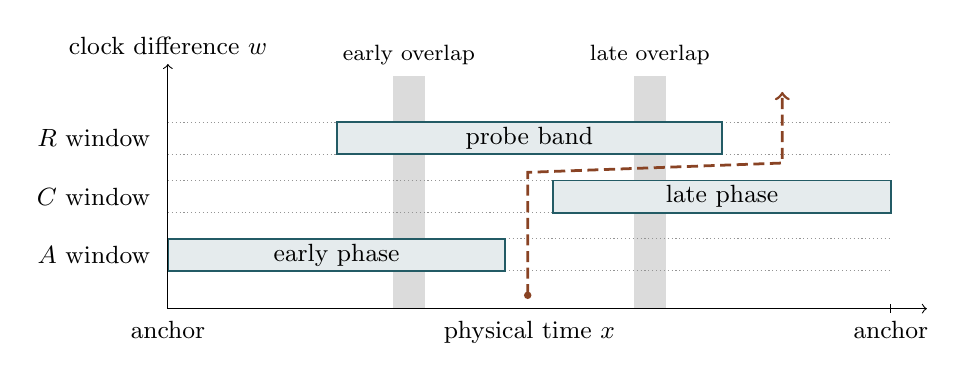
\begin{tikzpicture}[x=1.02cm,y=.74cm,font=\small,
  bar/.style={draw=episodeink,fill=episodeink!12,line width=.7pt},
  trace/.style={draw=episodetrace,line width=1pt,dash pattern=on 4pt off 2pt}]
  % A fixed bucket in one episode. Vertical strips are in x; rows are in w.
  \foreach \x in {2.8,5.8}{
    \fill[black!14] (\x,0) rectangle (\x+.4,4);
  }
  \foreach \y in {.65,1.65,2.65}{
    \draw[black!42,densely dotted] (0,\y) -- (9,\y);
    \draw[black!42,densely dotted] (0,\y+.55) -- (9,\y+.55);
  }

  \draw[bar] (0,.65) rectangle (4.2,1.20);
  \draw[bar] (4.8,1.65) rectangle (9,2.20);
  \draw[bar] (2.1,2.65) rectangle (6.9,3.20);
  \node at (2.10,.925) {early phase};
  \node at (6.90,1.925) {late phase};
  \node at (4.50,2.925) {probe band};
  \node[anchor=east] at (-.10,.925) {\(A\) window};
  \node[anchor=east] at (-.10,1.925) {\(C\) window};
  \node[anchor=east] at (-.10,2.925) {\(R\) window};

  \draw[trace,->] (4.48,.23) -- (4.48,2.34) -- (7.65,2.5) -- (7.65,3.72);
  \fill[episodetrace] (4.48,.23) circle (1.35pt);
  \draw[->] (0,0) -- (0,4.2) node[above] {clock difference \(w\)};
  \draw[->] (0,0) -- (9.45,0);
  \draw (9,.08) -- (9,-.08);
  \node[below] at (0,-.05) {anchor};
  \node[below] at (9,-.05) {anchor};
  \node[below] at (4.5,-.05) {physical time \(x\)};
  \node[anchor=south,font=\footnotesize] at (3.0,4.02) {early overlap};
  \node[anchor=south,font=\footnotesize] at (6.0,4.02) {late overlap};
\end{tikzpicture}
\caption{One bucket and one ordered triple of work windows. The rectangle
in each horizontal window marks the physical times when its transfer is
guaranteed. The dashed subpath spans the triple in \(w\) while missing all
three rectangles. Its \(x\)-coordinate traverses the shaded late overlap
as it moves from the \(C\) window to the \(R\) window.}
\label{fig:episode}
\end{figure}
